% !TEX root = ../thesis.tex
% testing and optimization experiments
% @author Tobias Wulf
%

\section{Verhalten bei kombinierten Fehllagen}\label{sec:exp6}

\textbf{Zweck:}

\textbf{Durchführung:}

\textbf{Erzeugte Datensätze:}

\textbf{Matlab-Skript:}

\textbf{Abweichende Parameter von \autoref{tab:sim-params-exp}:}

Abweichende Parameter:

Referenzposition (0,0,4.5) , 11deg 

\begin{itemize}
	\item TrainingsOptions: nAngles: 17
	\item TrainingsOptions/ TestOptions: xPos/ yPos: $(0;0)/(0,5;1)/(2,5;2)$
	\item TrainingsOptions/ TestOptions: zPos: $4,5$
	\item TrainingsOptions/ TestOptions: tilt: $11$
	\item GRPOptions: kernel : 'QFCAPX'
	\item $\sigma_f^2$-Bounds: $(0.4,20)$
	\item $\sigma_l$-Bounds: $(4,50)$
	\item $\sigma_n^2$-Bounds: $(3\cdot10^{-7},10^{-5})$
	\item GPROptions: mean: 'zero'
	\item OptimRuns 10
\end{itemize}

\textbf{Ergebnisse:}

\textbf{Beobachtungen:}


\clearpage
\begin{figure}[tbph]
	\centering
	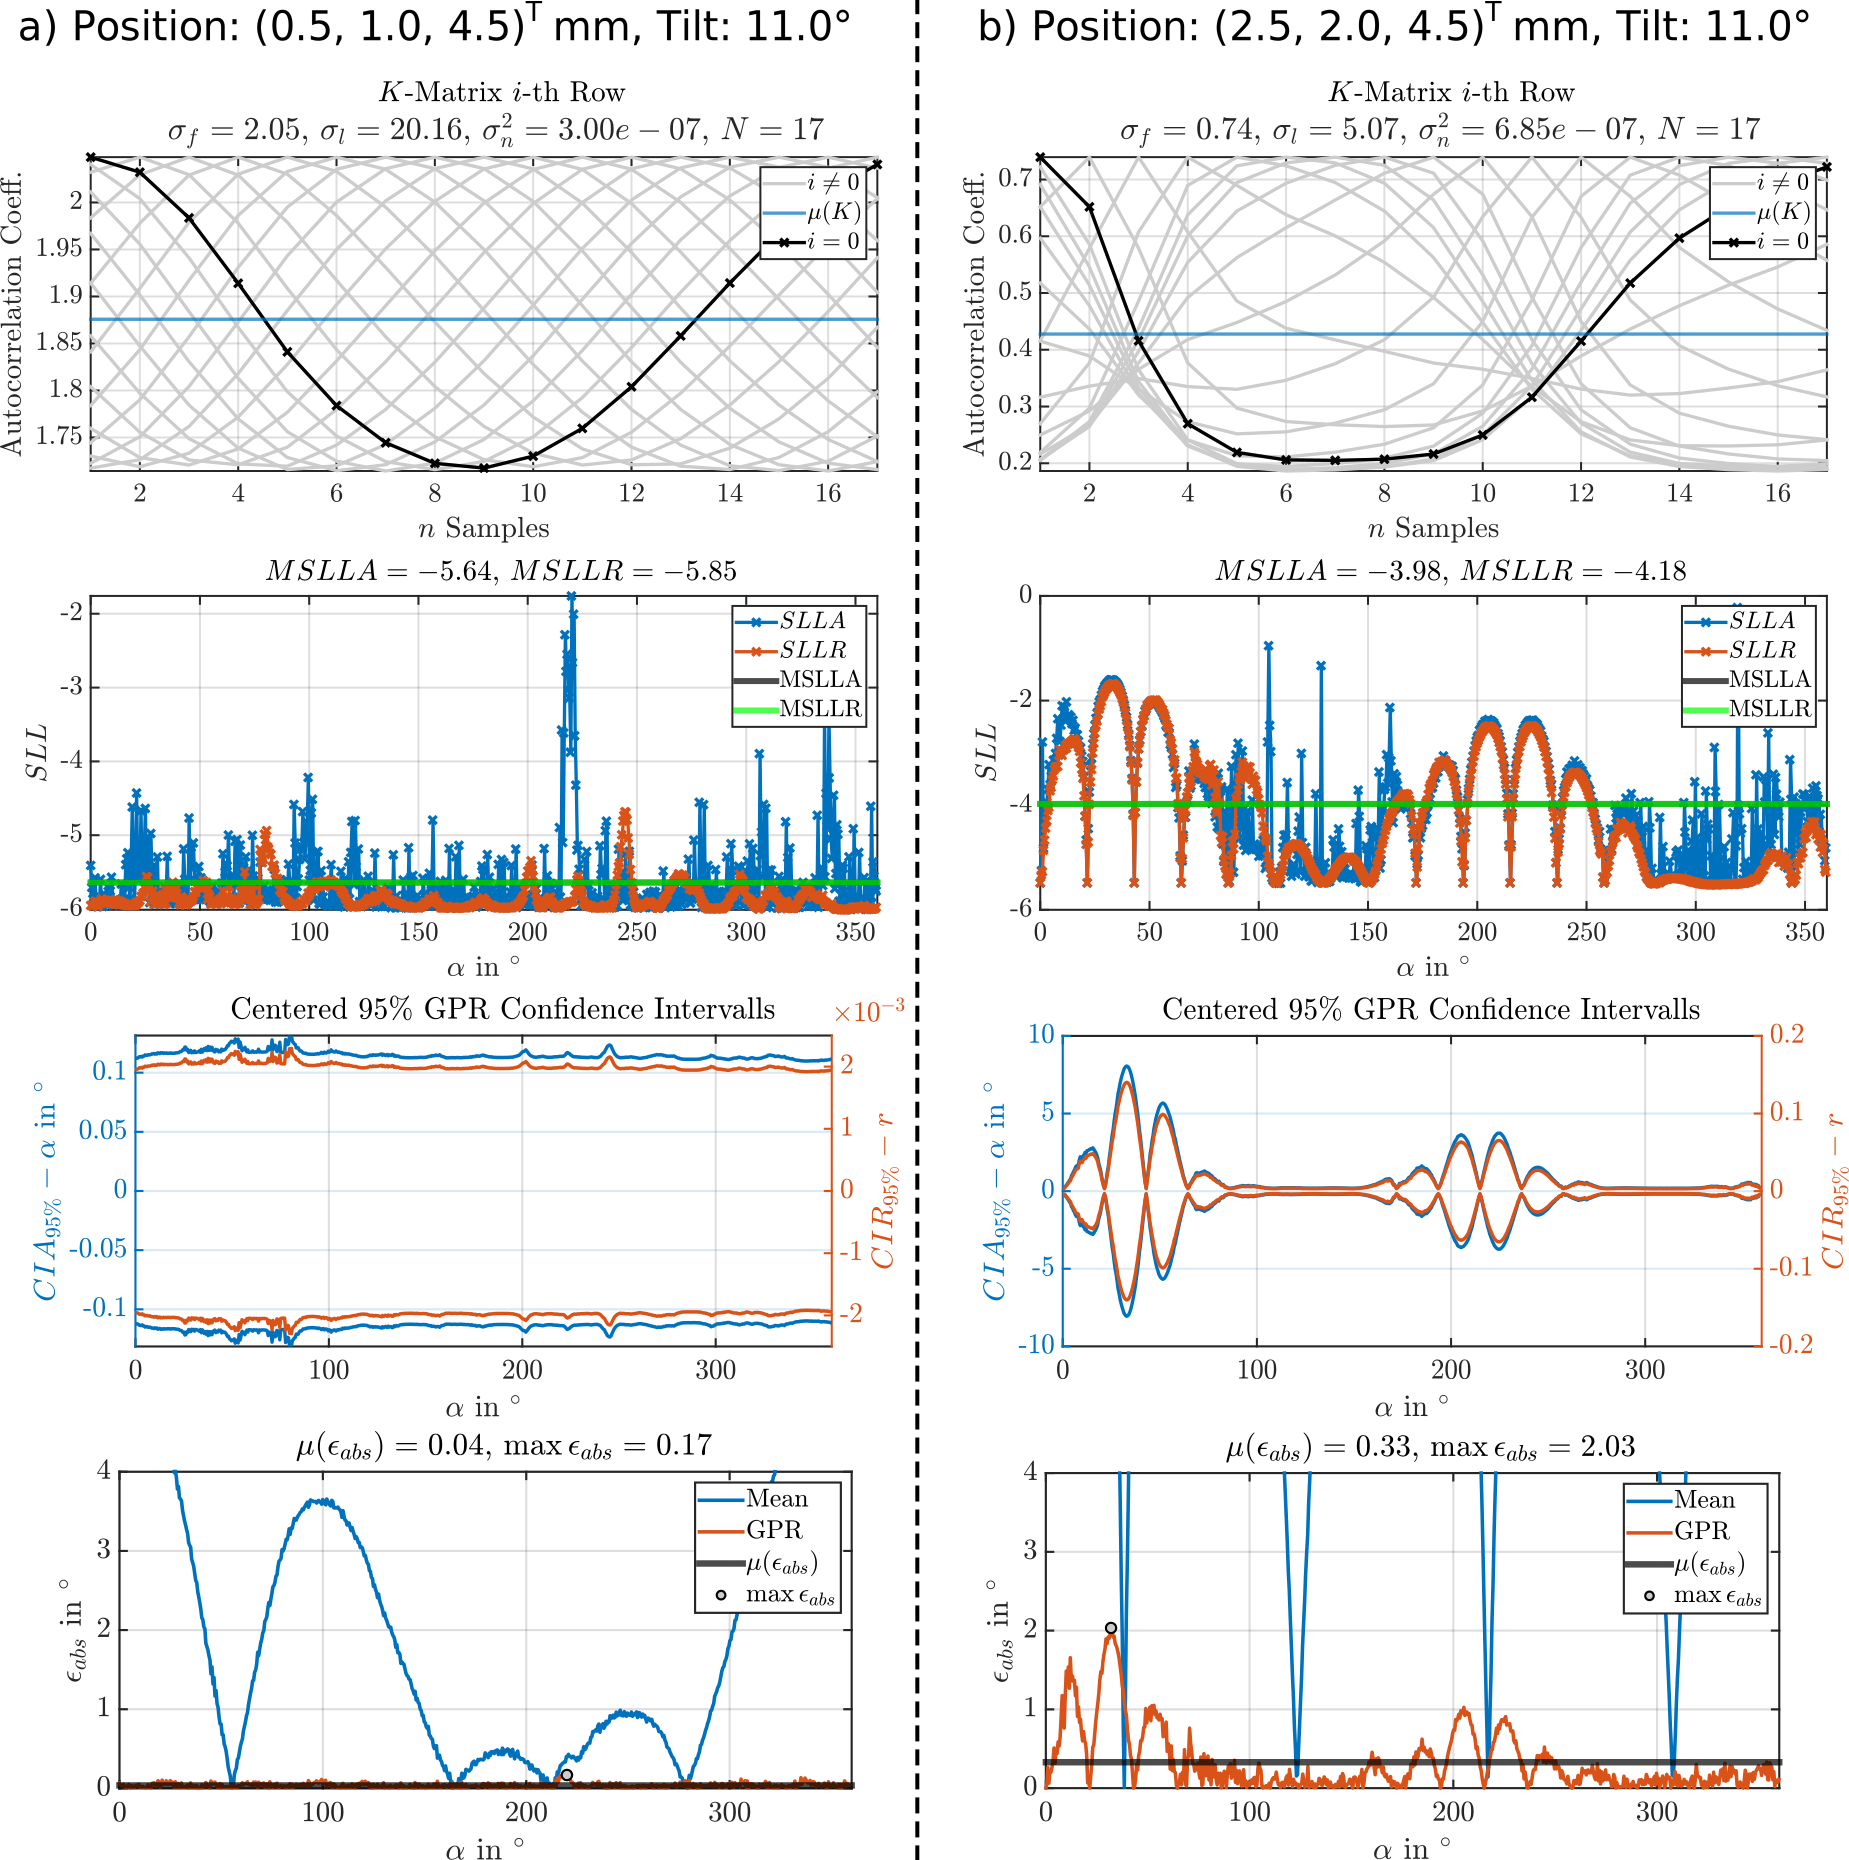
\includegraphics[width=\linewidth]{chapters/images/4-EuOExp/Kombinierte-Fehllagen-GPR}
	\caption[Kombinierte Fehllagen Modell]{Kombinierte Fehllagen Modell}
	\label{fig:kombinierte-fehllagen-gpr}
\end{figure}


\clearpage
\begin{landscape}
\begin{figure}[tbph]
	\centering
	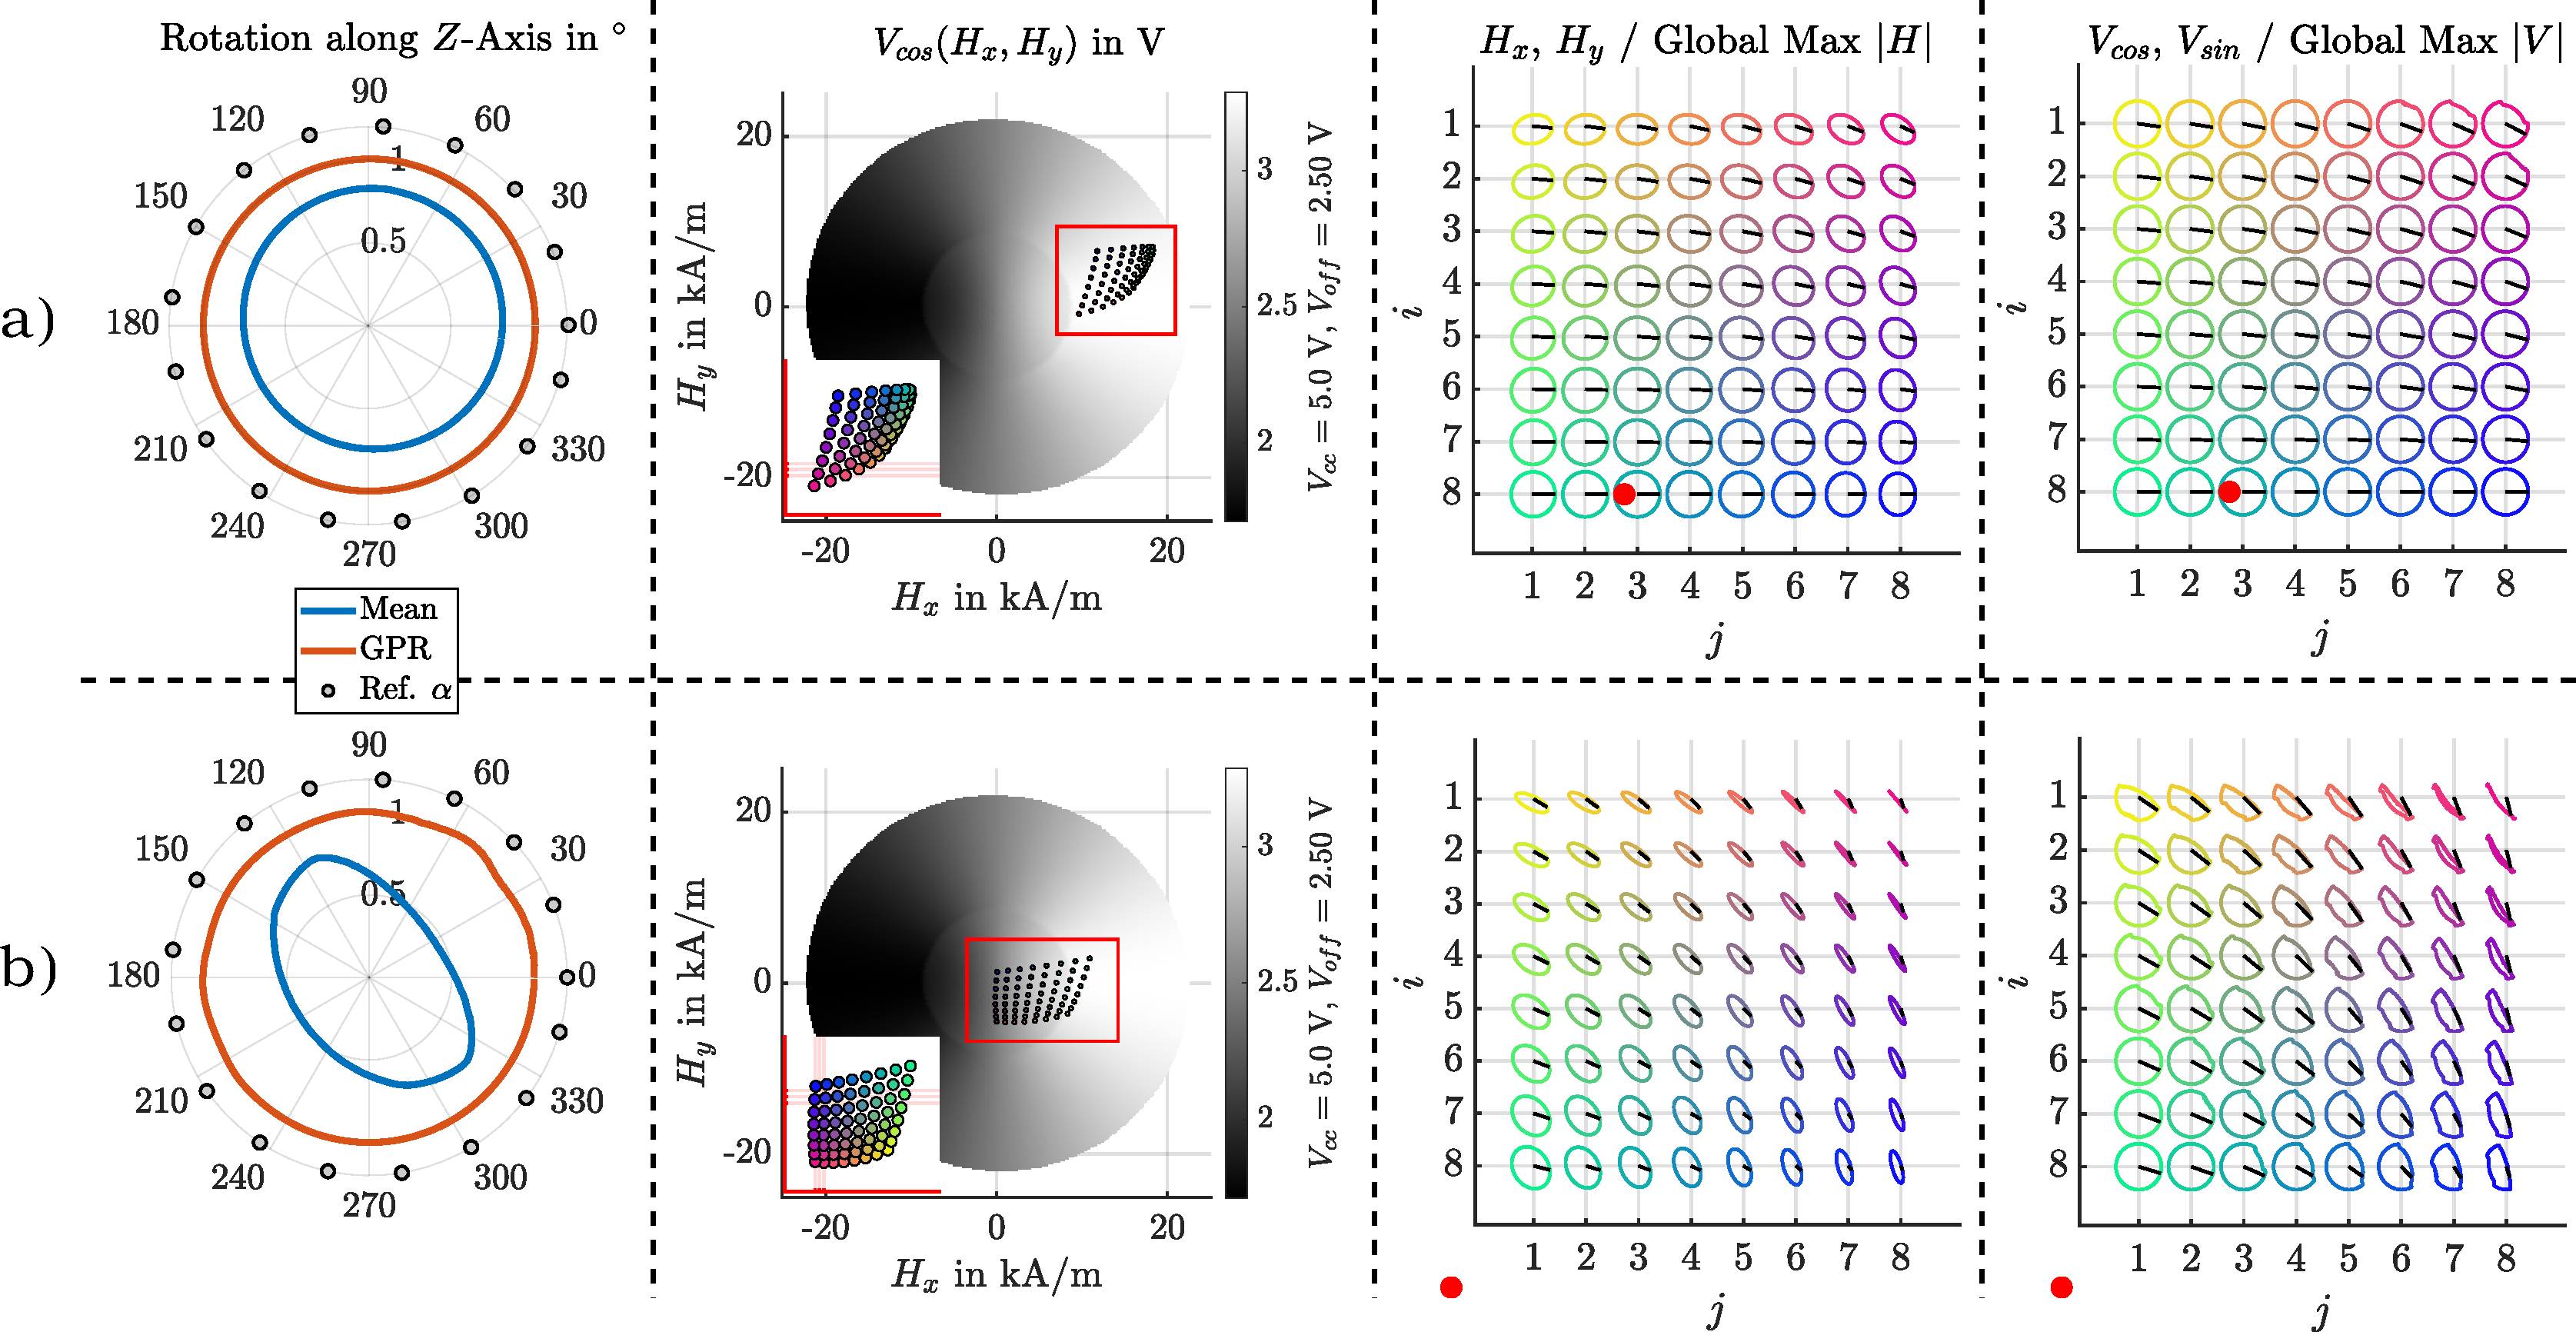
\includegraphics[width=\linewidth]{chapters/images/4-EuOExp/Kombinierte-Fehllagen-Sensor}
	\caption[Kombinierte Fehlagen Sensor]{Kombinierte Fehlagen Sensor beide 11 tilt a) (0,0,4.5) b) (2.5,2,4.5) Verzerrung}
	\label{fig:kombinierte-fehllagen-sensor}
\end{figure}	
\end{landscape}


\clearpage

